%!TEX root = ../thesis.tex
%*******************************************************************************
%*********************************** First Chapter *****************************
%*******************************************************************************

\chapter{Data-driven science}  %Title of the First Chapter
\label{chap:intro_stat}
\ifpdf
    \graphicspath{{Chapter1/Figs/Raster/}{Chapter1/Figs/PDF/}{Chapter1/Figs/}}
\else
    \graphicspath{{Chapter1/Figs/Vector/}{Chapter1/Figs/}}
\fi

\victor{This is a example of comment}

\cecile{This is a example of comment}

\isabelle{This is a example of comment}

\david{This is a example of comment}

\topic{This is a example of topic}
\content{This is a example of content}


\topic{Simulations combined with machine learning make possible to extract knowledge even in highly complex and stochastic process like High Energy Physics}

\content{Objectif : Improving the precision of parameter estimation in a special case of the inverse problem in the presence of systematic effect.}


\section{LHC experiments} % (fold)
\label{sec:lhc_experiments}

\topic{C'est très complexe mais on a pas besoin de toute cette complexité pour saisir le problème.}


\subsection{Counting problem} % (fold)
\label{sub:counting_problem}

\content{Short description of the physical system}
The system producing the data studied in this analysis is a particle collider.
Without getting into the details a particle collider is a machine accelerating small brick of matter, proton in this case, in oposite direction to smash them against each other.

\begin{figure}[htb]
    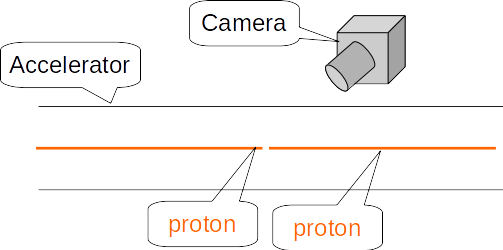
\includegraphics[width=\linewidth]{particle_collider_0}
    \caption{Very simple particle collider}
    \label{fig:particle_collider_0}
\end{figure}


\content{Soft / hard collision}

\begin{figure}[htb]
  \centering
  \begin{subfigure}[t]{0.49\linewidth}
    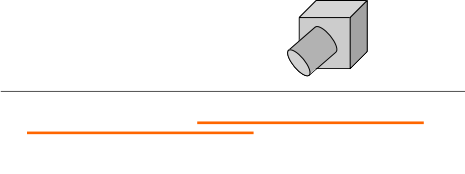
\includegraphics[width=\linewidth]{particle_collider_soft}
    \caption{soft collision}
    \label{fig:soft_collision}
  \end{subfigure}%
  \hfill
  \begin{subfigure}[t]{0.49\linewidth}
    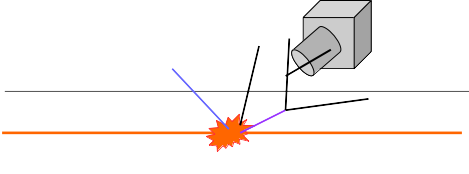
\includegraphics[width=\linewidth]{particle_collider_hard}
    \caption{hard collision}
    \label{fig:hard_collision}
  \end{subfigure}
  \caption{soft collision (left) and hard collision (right)}
  \label{fig:collision}
\end{figure}

\content{Explain what an event is}
\content{Introduce cross section estimations / mixture coefficient inference}
\content{This is a count problem. We want to estimate the amount of H to tau tau events}


\subsection{The model} % (fold)
\label{sub:the_model}

\content{Standard model to describe what happen.}
\content{Short description of the generative model}
\content{Simulation of the entire experiment}


\section{Inference through simulation} % (fold)
\label{sec:inference_through_simulation}

\victor{Or "Inference with/using simulations" ?}

\topic{Simulations/models are useful to explain data (therefore understand the undelying process that generated the data)}


\content{Dans un monde simple tout est "facile"}
\content{Introduire le problème d'extraction d'un coefficient de mélange(lié à cross-section)}

\subsection{Classic parameter estimation} % (fold)
\label{sub:classic_parameter_estimation}

\topic{Bayesian inference gives access to the full posterior}

\content{Introduce the basic statistics tools that we will use}
\content{Brute force method to do bayesian inference}
\content{Other (better) methods like variational inference}

Assuming that the likelihood $p(\theta | x)$ is available the Bayes theorem indicates how to access the posterior pobability.
$$
    p(\theta | x) = \frac{p(x|\theta) p(\theta)}{p(x)} = \frac{p(x|\theta) p(\theta)}{\int_\theta p(x|\theta) p(\theta)}
$$

The inference is then straitforward.
The prior $p(\theta)$ contains all the current knowledge about the problem. 
If no knowledge is available a non informative prior is chosen, usually a uniform distribution over the domain of $\theta$.
Computing $p(\theta | x)$ for the possible values $\theta$ \ie where the prior probability is not zero.
The integral on the denominator can either be computed by hand or approximated with Monte Carlo.


\topic{Maximum likelihood is more focused on what we are looking for (parameter estimation)}

\content{Maximum likelihood link to bayesian inference}
\content{Maximum likelihood gradient descent methods}
\content{Maximum likelihood variance estimation}





\subsection{Inverse problem} % (fold)
\label{sub:inverse_problem}

\topic{These methods don't scale to high dimensions}

\content{Computation complexity makes likelihood and posterior intractable}
\content{Numerical stability high dimensional integral ?}
\content{Maybe a "simple" example that shows how often in real life this setting may happen}

\topic{(another issue) Sometimes approximation needs to be made in order to build a simulation}

\content{Approximation requiered to build some part of LHC simulation as an example}
\victor{Very short subsection ?}
\content{Here or in the previous subsection : 1/2 page on the processes to simulate an event. In order to make clear how complicated it is.}


\subsection{Hand crafted dimension reduction} % (fold)
\label{sub:hand_crafted_dimension_reduction}

\topic{Ask a theorist to build a low dimensional feature}

\content{How it was done before machine learning}


\topic{Too many dimension ? Discard the less relevants ones}

\victor{Pas sûr que ça soit vraiment utilisé. Demander à David.}




\subsection{Count estimation} % (fold)
\label{sub:count_estimation}


\topic{Classifiers can achieve optimal inference}

\content{Proof of best estimator with bayesian classifier}
\content{Intuition of classifer as separator of population in order to compute a ratio}

\victor{Cette section reprend le papier de Neal \cite{Neal:2007zz}}

We are studying a stochatic phenomenon which generative process is described as :

\begin{equation}
	\label{eq:mixture_model}
	p(x|m) = m p(x|s) + (1-m) p(x|b)
\end{equation}
where $x$ is the set of observable features of the studied event gathered in a vector.
Events are split into 2 classes : the signals $S$ and the backgrounds $B$.
$m$ is the mixture coefficient between suignals and backgrounds.

$m$ can be seen as the probability for an event to be a signal $p(s)$. 
It naturally follows that $1-m$ is the probability for an event to be a background $p(b)=1-p(s)$.
\autoref{eq:mixture_model} can be written as
\begin{equation}
	p(x) = p(s)p(x|s) + p(b)p(x|b)
\end{equation}

In many interesting cases the nature of the event (signal/background) are not among the possible measurement that can be made.
Moreover the likelihoods $p(x|s)$ and $p(x|b)$ are intractable because of high dimension integrals or simply because computable formulas do not exist.
However building a simulator working only in forward mode allowing to sample from $p(x|m)$ is possible.
This problem is known as the inverse problem. 
The objective is to infer causal parameters from observations hence reversing the forward process which goes from causal parameters to observations.


The example that motivates this work is comming from High Energy Physics (HEP) where events are collisions in a particle accelerator.
Signals are events giving birth to a Higgs boson and backgrounds gather all the other collisions.
$m$ is therefore connected to branch factor (cross section ?) of the Higgs boson which is the parameter we want to measure.

\victor{Link between cross-section, branch factor, luminosity ?}

Measurements are made from a large bunch of independant and identically distributed events $D=\{x_i\}_{i=1}^N$.

\begin{align*}
	p(D|m) =& \prod_{i=1}^N m p(x|s) + (1-m) p(x|b) \\
	       =& \prod_{i=1}^N p(x|b) \left [(1-m) + m \frac{p(x|s)}{p(x|b)} \right ]\\
	       =& \underbrace{\left[ \prod_{i=1}^N p(x|b) \right ]}_{h(x)} \times 
	       \underbrace{\left [\prod_{i=1}^N (1-m) + m \frac{p(x|s)}{p(x|b)} \right ]}_{g_m(T(x))}
\end{align*}
with $T(x) = \frac{p(x|s)}{p(x|b)} $

Fisher-Neyman factorization theorem states that $T(x)$ is a sufficient summary statistic to obtain $m$

The maximum likelihood estimator, noted $\hat m$ is commonly used to estimate the parameter of interest.
Recall that maximum likelihood estimator are strictly equivalent to a maximum a posteriori estimator using a uniform prior.
This is a reasonable choice when we do not have prior knowledge as in this example.

\begin{equation}
	\hat m = \argmax_m p(m | D)
\end{equation}

It is more convenient (numerical stability) to express the result as a deviation from the prediction of the Standard Model.
The deviation is defined as :

\begin{equation}
	\mu = \frac{p(s)}{p_{SM}(s)} = \frac{m}{p_{SM}(s)}
\end{equation}
$p_{SM}(s)$ is the expected probability to get a signal following the Standard Model.
Recovering $m$ from $\mu$ is trivially done with $m = \mu p_{SM}(s)$.

The estimator is now :
\begin{align}
	\hmu =& \argmax_\mu p(\mu | D) \\
	     =& \argmax_\mu \frac{p(\mu)}{p(D)} p(D | \mu) \\
	     =& \argmax_\mu p(\mu) p(D | \mu) \\
	     =& \argmax_\mu  p(D | \mu) \\
	     =& \argmax_\mu  \prod_{i=1}^N g_\mu(T(x)) \\
\end{align}


$T(x)$ can be obtained using a classifier $c$ trained to separate signals and backgrounds.
A Bayes optimal classifier output gives :
\begin{equation}
	c(x) = \frac{s p(x|s)}{(1-s) p(x|b) + s p(x|s)}
\end{equation}
where $s$ is the fraction of signals used in the training dataset.

\begin{equation}
	T(x) = \frac{c(x)}{(1-c(x))} \frac{(1-s)}{s} 
\end{equation}


Note : $c$ is also a sufficient summary statistic
\begin{equation}
	g_\mu(T(x)) = 1 - \mu p_{SM}(s) + \mu p_{SM}(s) \times \frac{c(x)}{(1-c(x))} \frac{(1-s)}{s} = f_\mu(c(x))
\end{equation}

\content{Limitation : what happens if the classifier is not (Bayes) optimal ? Can we detect it ?}
\content{Physicis alos uses the Neyman-Pearson theorem on statistical test to justify maximum likelihood estimator usage. Should I include it here ? or in \autoref{sub:maximum_likelihood} ?}



\subsection{Poisson distribution} % (fold)
\label{sub:poisson_distribution}

\content{Comment on passe du ratio de vraissemblance du classifier à Poisson}

On a plein de processus binomiaux et un théorème indiquant que la loi de Poisson est une excelente approximation quand on a plein de points.

Donc le nombre d'events dans une boite donnée suit une loi de Poisson.
\begin{equation}
	n \sim Poisson(\mu s + b)
\end{equation}

\begin{equation}
	P(n| \mu, s, b) = \frac{(\mu s +b)^n }{n!} e^{-(\mu s + b)}
\end{equation}

$s$ et $b$ sont des sorties du modèle calculer avec le classifieur sur la simulation.
C'est ça le lien. Mais pourquoi c'est comme ça ?


\content{Binned Poisson to increase Sig/Bkg}


\subsection{Workflow} % (fold)
\label{sub:workflow}

\topic{In real life we do both mathematical models + machine learning.}
\victor{Meaning : computing hand crafted features to reduce from $\RR^{100 000}$ to $\RR^{40}$ then using machine learning to reduce to $\RR$}

\content{We don't need ML when we know how to write the code to compute features}
\content{We use ML when we don't know how to write the code}
\content{Clin d'oeil au tracking. On a le code mais le faire passer à l'échelle reste très difficile.}
\content{Schéma du workflow pour calculer notre estimateur}


\section{Systematic effects} % (fold)
\label{sec:systematic_effects}

\topic{Systematic effects make inference more complex by introducing nuisance parameters}



\subsection{Definition} % (fold)
\label{sub:definition}

\content{Definition and example of systematic effects (not only in HEP !)}
\victor{Laisser le lecteur penser de lui même à l'adaptation de domaine.}

Définition de la variance :

$\VV(Y) = \EE[(Y - \EE[Y])^2] = \EE(Y^2) - [\EE(Y)]^2$

Théorème de la variance totale \needcite :

\begin{eqnarray}
    \VV[Y] =& \EE_X \left (\VV[Y|X] \right ) &+ \VV_X \left (\EE[Y|X]\right ) \\
    \VV[Y] =& \EE_X \left (\VV[Y|X] \right ) &+ \EE_X \left ( (\EE [Y|X]  - \EE[Y])^2\right )
\end{eqnarray}


En remplaçant la v.a. $Y$ par $y|x$ et $X$ par $\alpha$ on obtient :

$$
\VV[y|x] = \EE_{\alpha \sim p(\alpha|x)} \left (\VV[y|x, \alpha] \right ) + \EE_{\alpha \sim p(\alpha|x)} \left ( (\EE [y|x, \alpha]  - \EE[y|x])^2\right )
$$


On dirait presque que : 
$$\EE_{\alpha \sim p(\alpha|x)} \left ((\EE [y|x, \alpha]  - \EE[y|x])^2\right )$$
représente l'erreur systématique. 
Car c'est l'écart de notre estimation de $y$ sachant $x$ et $\alpha$ par rapport à la moyenne.
Surtout, si $\alpha|x$ est parfaitement connu (ie c'est un dirac) alors ce terme s'annule !

Mais je ne suis pas sûr que l'on puisse dire que
$$\EE_{\alpha \sim p(\alpha|x)} \left (\VV[y|x, \alpha] \right )$$
représente l'erreur statistique.

Mais si ça marche on aurrait une définition claire et précise de ce qu'est l'erreur statistique et l'erreur systématique.


\content{Schéma inverse problem with nuisance parameters}

\subsection{Classifier optimality} % (fold)
\label{sub:classifier_optimality}

\topic{Systematic effect breaks the optimality of the classifier}

\content{Why the proof does not work anymore}

\content{Poisson likelihood is not broken but weakened}

\subsection{Variance estimations} % (fold)
\label{sub:variance_estimations}

\topic{We can measure the effect of systematics on the final variance (inference is still possible)}

\content{On a caché ça sous le tapis jusqu'à maintenant mais c'est le coeur du sujet !}
\content{It does not "breaks" it but increase the variance/uncertainty}
\content{Introduce systematic vs statistical uncertainty as the 2 component of the variance}
\content{Glen's formulas ?}

\content{Marginalization could do the job but is computationally expensive}


\subsection{Profiled likelihood} % (fold)
\label{sub:profiled_likelihood}

\topic{The current way of measuring the variance of our estimation to include systematics is "profiled likelihood"}

\content{Explain how profiled likelihood works and why is works}
\content{Introduce Fisher information matrix and Cramer Rao bound (since we will use it later for INFERNO)}




\subsection{Looking for better} % (fold)
\label{sub:looking_for_better}

\topic{This document is about going further than the "simple" classifier method}

\content{Annonce de la suite / du plan du manuscrit}


